\documentclass[t,dvipsnames]{beamer}
\usepackage{mathtools}
\usepackage{siunitx}
\usepackage[T1]{fontenc}
\usepackage[sfdefault,lining,scaled=.85]{FiraSans}
\usepackage[scaled=0.85]{FiraMono}
\usepackage{newtxsf}

% https://tex.stackexchange.com/questions/435376
\makeatletter
\re@DeclareMathSymbol{\br@cext}{\mathord}{largesymbolsTXA}{32}
\makeatother

\usepackage{pifont}
\usepackage[utf8]{inputenc}
\usepackage{mdwlist}
\usepackage{hyperref}

\usetheme{UAmnf}

\setbeamerfont{frametitle}{family=\sffamily\firamedium}
\setbeamercolor{frametitle}{fg=white}
\setbeamertemplate{navigation symbols}{}
\setbeamertemplate{headline}{  
  \leavevmode
   \begin{beamercolorbox}{logo in headline}
	\includegraphics[width=\paperwidth]{UA_mnf_headline}
   \end{beamercolorbox}
}
\setbeamercolor{alerted text}{fg=red!70!black}
\renewcommand\mathfamilydefault{\rmdefault}

\hypersetup{%
  pdftitle={Introduction to Feynman path integrals}
  ,pdfauthor={Gert-Ludwig Ingold}
  ,pdfsubject={Presentation at the Bad Honnef Physics School on
	       Methods of Path Integration in Modern Physics, Bad Honnef, 25.8.2019}
  ,pdfkeywords={Feynman path integrals, propagator, particle in a box,
                particle on a ring, harmonic oscillator}
}

\graphicspath{{./img/}}

\title[Introduction to Feynman path integrals]%
      {Introduction to Feynman path integrals}

\begin{document}

\begin{frame}[t]{}
 \vspace{2.0truecm}
 \begin{center}
   \structure{\LARGE\firamedium Introduction to Feynman path integrals}\\[0.2truecm]

   \vspace{0.1truecm}
   {\Large Gert-Ludwig Ingold}

   {\large Universität Augsburg}

   \vspace{3.4truecm}
   {\scriptsize Bad Honnef Physics School on \textit{Methods of Path Integration in
    Modern Physics}, 25.--31.8.2019}
 \end{center}
\end{frame}

\navtrue

\section{Motivation}

\begin{frame}[c]{}
 \begin{center}
  \begin{minipage}{0.8\textwidth}
   \only<1>{\tableofcontents}%
   \only<2>{\tableofcontents[currentsection]}%
  \end{minipage}
 \end{center}
\end{frame}

\begin{frame}[t]{Classical mechanics: Hamilton vs. Lagrange}

 \vspace{-0.5truecm}
 \begin{columns}
  \begin{column}[t]{0.5\textwidth}
   \begin{center}
    \textbf{Hamilton formalism}

    Hamiltonian $H(q, p)$

    \vspace{0.2truecm}
    Poisson bracket $\{q, p\} = 1$

    equations of motion $\dot q = \{q, H\}, \dot p = \{p, H\}$
   \end{center}
  \end{column}%
  \begin{column}[t]{0.5\textwidth}
   \begin{center}
    \textbf{Lagrange formalism}

    Lagrangian $L(q, \dot q)$

    \vspace{0.2truecm}
    action $S = \int\text{d}t L(q, \dot q)$

    equation of motion from Hamilton's principle $\delta S = 0$

   \end{center}
  \end{column}%
 \end{columns}

 \begin{columns}
  \begin{column}[t]{0.5\textwidth}
   \begin{center}
    $\Arrowvert$

    canonical quantization $[\hat q, \hat p] = \text{i}\hbar$

    $\Downarrow$
   \end{center}
  \end{column}%
  \begin{column}[t]{0.5\textwidth}
   \begin{center}
    $\Arrowvert$

    ?

    $\Downarrow$
   \end{center}
  \end{column}%
 \end{columns}

 \begin{columns}
  \begin{column}[t]{0.5\textwidth}
   \begin{center}
   Heisenberg, Schrödinger, \ldots (1925)

   Schrödinger equation $\hat H\vert\Psi\rangle =
	  \text{i}\hbar\frac{\partial}{\partial t}\vert\Psi\rangle$ 
   \end{center}
  \end{column}%
  \begin{column}[t]{0.5\textwidth}
   \begin{center}
    Dirac (1933), Feynman (1948)

    \vspace{0.2truecm}
    \fcolorbox{red!70!black}{red!10}{%
       \begin{minipage}{0.75\textwidth}
	\begin{center}
         \alert{Path integral formulation of quantum mechanics}
	\end{center}
       \end{minipage}
    }
   \end{center}
  \end{column}%
 \end{columns}
\end{frame}

\begin{frame}[c]{Why base quantum mechanics\\ on Lagrange formalism?}
 path integral formulation of quantum mechanics \ldots
 \begin{itemize}
  \item \ldots can provide an alternative view on physical problems
  \item \ldots does without operators\\
	for fermionic fields, Grassmann variables are used
  \item \ldots is very well suited for relativistic field theories\\[0.2truecm]
	action $S=\int\text{d}^4x\mathcal{L}(\phi, \partial_\mu\phi)$
		 is a Minkowski scalar\\[0.2truecm]
	Hamiltonian density $\mathcal{H}(\phi, \pi)$ corresponds to the
	$0-0$ component of the energy-momentum tensor
  \item \ldots is very well suited to consider the semiclassical limit
	$S\gg\hbar$
 \end{itemize}
\end{frame}

\section{Propagator}

\begin{frame}[c]{}
 \begin{center}
  \begin{minipage}{0.8\textwidth}
   \tableofcontents[currentsection]
  \end{minipage}
 \end{center}
\end{frame}

\begin{frame}[t]{Propagator}
 Schrödinger equation\quad
 $\text{i}\hbar\dfrac{\partial}{\partial t}\vert\Psi(t)\rangle = H\vert\Psi(t)\rangle$

 \vspace{0.5truecm}
 time evolution of a state
 \begin{displaymath}
  \vert\Psi(t)\rangle = U(t)\vert\Psi(0)\rangle\quad \text{with}\quad
  U(t) = \exp\left(-\frac{\text{i}}{\hbar}Ht\right)
 \end{displaymath}
 in position representation
 \begin{displaymath}
  \textcolor{blue}{\langle q_\text{f}}\vert\Psi(t)\rangle =
   \textcolor{green!40!black}{\int\!\!\text{d}q_\text{i}}\textcolor{blue}{\langle q_\text{f}\vert}
   U(t)\textcolor{green!40!black}{\vert q_\text{i}\rangle\langle q_\text{i}}\vert\Psi(0)\rangle
 \end{displaymath}
 \begin{displaymath}
  \Psi(q_\text{f}, t) = \int\text{d}q_\text{i} K(q_\text{f}, q_\text{i}, t)\Psi(q_\text{i}, 0)
 \end{displaymath}

 \vspace{0.5truecm}
 \structure{$\Rightarrow$\quad propagator\quad
	    $K(q_\text{f}, q_\text{i}, t) = \langle q_\text{f}\vert U(t)\vert q_\text{i}\rangle$}
\end{frame}

\begin{frame}[c]{Propagator of a free particle}
 Hamiltonian of the free particle\qquad $H = \dfrac{p^2}{2m}$

 \vspace{0.5truecm}
 propagator of the free particle
 \begin{displaymath}
  \begin{aligned}
  K(q_\text{f}, q_\text{i}, t) &= \langle q_\text{f}\vert\text{e}^{-\frac{\text{i}}{\hbar}Ht}
                                   \vert q_\text{i}\rangle\\
     &= \int_{-\infty}^{+\infty}\text{d}p\langle q_\text{f}\vert p\rangle\langle p\vert q_\text{i}\rangle
	  \text{e}^{-\frac{\text{i}}{\hbar}\frac{p^2}{2m}t}\\
     &= \frac{1}{2\pi\hbar}\int_{-\infty}^{+\infty}\text{d}p
          \exp\left[-\dfrac{\text{i}}{\hbar}\left(\dfrac{p^2}{2m}t-(q_\text{f}-q_\text{i})p\right)\right]\\
     &= \frac{1}{2\pi\hbar}\exp\left(\frac{\text{i}}{\hbar}\frac{m(q_\text{f}-q_\text{i})^2}{2t}\right)
	  \int_{-\infty}^{+\infty}\text{d}p\exp\left(-\frac{\text{i}}{\hbar}\frac{t}{2m}p^2\right)
  \end{aligned}
 \end{displaymath}
\end{frame}

\begin{frame}[c]{Digression: Fresnel integral}
 \begin{columns}
  \begin{column}[b]{0.5\textwidth}
   \begin{displaymath}
    \begin{aligned}
     \int_0^\infty\text{d}x\text{e}^{\text{i}\alpha x^2}
          &= \text{e}^{\text{i}\pi/4}\!\int_0^\infty\!\text{d}u\text{e}^{-\alpha u^2}\\
          &= \frac{1}{2}\sqrt{\frac{\text{i}\pi}{\alpha}}
    \end{aligned}
   \end{displaymath}

   \begin{displaymath}
    \Rightarrow\int_{-\infty}^{+\infty}\text{d}x\text{e}^{-\text{i}\alpha x^2}
          = \sqrt{\frac{\pi}{\text{i}\alpha}}
   \end{displaymath}

  \end{column}%
  \begin{column}[b]{0.5\textwidth}
   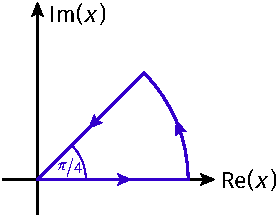
\includegraphics[width=\textwidth]{fresnel}

   \vspace{-0.4truecm}
  \end{column}
 \end{columns}
\end{frame}

\begin{frame}[c]{Propagator of a free particle and\\ relation to classical properties}
 propagator 
 \begin{displaymath}
  K(q_\text{f}, q_\text{i}, t) = \langle q_\text{f}\vert\text{e}^{-\frac{\text{i}}{\hbar}Ht}
                                   \vert q_\text{i}\rangle
     = \sqrt{\frac{m}{2\pi\text{i}\hbar t}}\exp\left(\frac{\text{i}}{\hbar}
	    \frac{m(q_\text{f}-q_\text{i})^2}{2t}\right)
 \end{displaymath}

 \vspace{0.3truecm}
 classical motion from position $q_\text{i}$ to $q_\text{f}$ in time $t$:
 \begin{itemize}
  \item classical path\quad $q(s) = q_\text{i} + (q_\text{f}-q_\text{i})\dfrac{s}{t}$
  \item classical action\quad
	$S_\text{cl} = \int_0^t\text{d}s\dfrac{m}{2}\dot q^2
		     = \dfrac{m(q_\text{f}-q_\text{i})^2}{2t}$
 \end{itemize}

 \vspace{0.4truecm}
 propagator of free particle in terms of classical properties

 \begin{center}
  \fcolorbox{red!70!black}{red!10}{\alert{%
  $K(q_\text{f}, q_\text{i}, t) = \sqrt{-\dfrac{1}{2\pi\text{i}\hbar}
	 \dfrac{\partial^2 S_{cl}}{\partial q_\text{i}\partial q_\text{f}}}
	 \exp\left(\dfrac{\text{i}}{\hbar}S_\text{cl}\right)$
  }}
 \end{center}
\end{frame}

\begin{frame}[c]{Combining two propagators}
 semigroup property
 \begin{displaymath}
  \begin{aligned}
   K(q_\text{f}, q_\text{i}, t_2+t_1) &= \langle q_\text{f}\vert
	  \text{e}^{-\frac{\text{i}}{\hbar}Ht_2}
	  \text{e}^{-\frac{\text{i}}{\hbar}Ht_1}\vert q_\text{i}\rangle\\
     &= \textcolor{blue}{\int_{-\infty}^{+\infty}\text{d}q'}\langle q_\text{f}\vert
	  \text{e}^{-\frac{\text{i}}{\hbar}Ht_2}\textcolor{blue}{\vert q'\rangle\langle q'\vert}
	  \text{e}^{-\frac{\text{i}}{\hbar}Ht_1}\vert q_\text{i}\rangle\\
     &= \int_{-\infty}^{+\infty}\text{d}q' K(q_\text{f}, q', t_2)K(q', q_\text{i}, t_1)
  \end{aligned}
 \end{displaymath}

 \begin{columns}
  \begin{column}[b]{0.4\textwidth}
   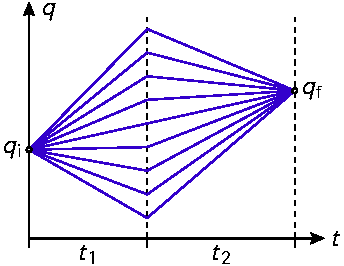
\includegraphics[width=\textwidth]{semigroup}
  \end{column}%
  \begin{column}[b]{0.6\textwidth}
   \begin{center}
   \fbox{%
    \begin{minipage}{0.8\textwidth}
     \textit{Exercise:} Check the semigroup property for the propagator of a free particle.
    \end{minipage}}
   \end{center}

   \vspace{0.8truecm}
  \end{column}
 \end{columns}
\end{frame}

\section{Derivation of path integral}

\begin{frame}[c]{}
 \begin{center}
  \begin{minipage}{0.8\textwidth}
   \tableofcontents[currentsection]
  \end{minipage}
 \end{center}
\end{frame}

\begin{frame}[c]{Strategy for the derivation of the\\
	         Feynman path integral}
 basic steps:
 \begin{itemize}
  \item use semigroup property to split the propagator into
	a large number of short-time propagators
  \item use the Baker-Campbell-Hausdorff formula to separate
	kinetic and potential contributions to the Hamiltonian
        in the time-evolution operator
 \end{itemize}
\end{frame}

\begin{frame}[c]{Baker-Campbell-Hausdorff formula\\
	         and Lie-Trotter formula}
 application to a short-time propagator with operators $T$ and
 $V$ representing kinetic and potential energy, respectively
 \begin{displaymath}
   \exp\!\left(-\frac{\text{i}}{\hbar}(T+V)\Delta t\right)
	  = \exp\!\left(-\frac{\text{i}}{\hbar}V\Delta t\right)
	     \exp\!\left(-\frac{\text{i}}{\hbar}T\Delta t\right)
	     \exp\!\left(-\frac{\text{i}}{\hbar^2}X\Delta t^2\right)
 \end{displaymath}
 \begin{displaymath}
  X = \frac{\text{i}}{2}[V,T]
      -\frac{1}{6\hbar}\bigg([V,[V,T]]-2[T,[T,V]]\bigg)\Delta t+\ldots
 \end{displaymath}

 \vspace{0.3truecm}
 for $\Delta t\to 0$, the last factor may be neglected

 \structure{$\Rightarrow$ Lie-Trotter formula}
 \begin{displaymath}
  \exp\!\left(-\frac{\text{i}}{\hbar}(T+V)t\right) =
    \lim_{N\to\infty}\left[\exp\!\left(-\frac{\text{i}}{\hbar}V\frac{t}{N}\right)
      \exp\!\left(-\frac{\text{i}}{\hbar}T\frac{t}{N}\right)\right]^N
 \end{displaymath}
\end{frame}

\begin{frame}[c]{Splitting the propagator I}
 propagator\qquad $\Delta t=\dfrac{t}{N}\quad q_0=q_\text{i}\quad q_N=q_\text{f}$
 \begin{multline*}
  \hspace{-0.5truecm}\langle q_\text{f}\vert U(t)\vert q_\text{i}\rangle =\\
  \int_{-\infty}^{+\infty}\left(\prod_{n=1}^{N-1}\text{d}q_n\right)
    \langle q_\text{f}\vert \cdots\vert q_n\rangle\underbrace{\langle q_n\vert
	 \text{e}^{-\frac{\text{i}}{\hbar}V\Delta t}
	 \text{e}^{-\frac{\text{i}}{\hbar}T\Delta t}
	 \vert q_{n-1}\rangle}_{\mathclap{\text{\small $%
	 \sqrt{\frac{m}{2\pi\text{i}\hbar\Delta t}}\exp\left[\frac{\text{i}}{\hbar}
	 \left(\frac{m(q_n-q_{n-1})^2}{2\Delta t}-V(q_n)\Delta t\right)\right]$}}}
	 \langle q_{n-1}\vert\cdots\vert q_\text{i}\rangle
 \end{multline*}
 \begin{center}
  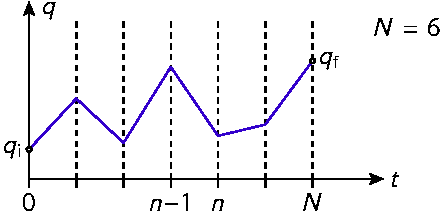
\includegraphics[width=0.6\textwidth]{splitting}
 \end{center}
\end{frame}

\begin{frame}[c]{Splitting the propagator II}
 \begin{multline*}
  \langle q_\text{f}\vert U(t)\vert q_\text{i}\rangle
  = \sqrt{\frac{m}{2\pi\text{i}\hbar\Delta t}}\int_{-\infty}^{+\infty}
    \prod_{n=1}^{N-1}\left(\sqrt{\frac{m}{2\pi\text{i}\hbar\Delta t}}\text{d}q_n\right)\\
    \times\exp\left[\frac{\text{i}}{\hbar}\sum_{n=1}^N\left(
	 \frac{m}{2}\bigg(\frac{q_n-q_{n-1}}{\Delta t}\bigg)^2
	 -V(q_n)\right)\Delta t\right]
 \end{multline*}
 \begin{center}
  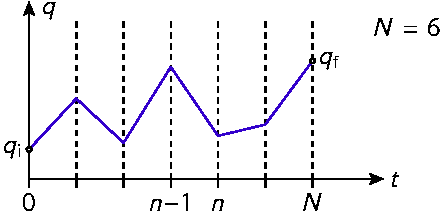
\includegraphics[width=0.6\textwidth]{splitting}
 \end{center}

 \vspace{0.5truecm}
 \begin{center}
  let us now take the continuum limit $N\to\infty$
 \end{center}
\end{frame}

\begin{frame}[c]{Action}
 \begin{displaymath}
  \lim_{N\to\infty}\sum_{n=1}^N\left(\frac{m}{2}\bigg(\frac{q_n-q_{n-1}}{\Delta t}\bigg)^2
                                     -V(q_n)\right)\Delta t
	= \int_0^t\text{d}s\left(\frac{m}{2}\dot q(s)-V(q)\right)
 \end{displaymath}

 in the exponent of the propagator, we find the action functional
 \begin{displaymath}
  S[q] = \int_0^t\text{d}s\left(\frac{m}{2}\dot q(s)-V\big(q(s)\big)\right)
 \end{displaymath}
 which takes a function $q(s)$ and returns a number $S$

 \begin{center}
  \structure{%
  $\Rightarrow$\quad%
  \begin{minipage}[t]{0.7\textwidth}
   \raggedright we have obtained a connection between the Lagrange formalism
   of classical mechanics and the quantum mechanical propagator
  \end{minipage}}
 \end{center}
\end{frame}

\begin{frame}[c]{Feynman path integral}
 propagator as functional integral (Feynman path integral)

 \begin{center}
  \fcolorbox{red!70!black}{red!10}{\alert{%
    $\displaystyle K(q_\text{f}, q_\text{i}, t) = \int_{q(0)=q_\text{i}}^{q(t)=q_\text{f}}\mathcal{D}q\,
    exp\left(\frac{\text{i}}{\hbar}S[q]\right)$
  }}
 \end{center}

 \vspace{0.5truecm}
 the integral runs over all trajectories $q(s)$ satisfying the boundary
 conditions $q(0)=q_\text{i}$ and $q(t)=q_\text{f}$

 \begin{center}
  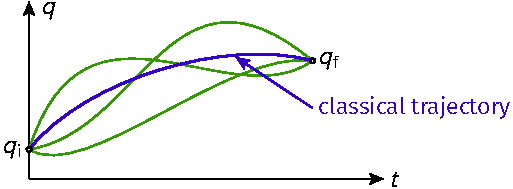
\includegraphics[width=0.8\textwidth]{feynman}
 \end{center}
\end{frame}

\begin{frame}[c]{Evaluation of a Feynman path integral}
 \begin{itemize}
  \item evaluate discretized version as an $N$-dimensional integral\\
	for linear systems, the following relation is useful:
	\begin{displaymath}
	 \int_{-\infty}^{+\infty}\text{d}x^N \exp\left(-\mathbf{x}^\text{T}
	    \mathbf{A}\hspace{0.1em}\mathbf{x}\right) =
		\sqrt{\frac{\pi^N}{\det(\mathbf{A})}}
	\end{displaymath}
  \item expansion in a complete set of functions\\
	$\rightarrow$ see our later discussion of the harmonic oscillator
 \end{itemize}

 \vspace{0.5truecm}
 \begin{center}
 \fbox{%
  \begin{minipage}{0.75\textwidth}
   \textit{Exercise:} Evaluate the Feynman path integral for the free particle
   by means of discretization. Why is the result independent of $N$?
  \end{minipage}}
 \end{center}
\end{frame}

\begin{frame}[t]{Physical interpretation}
 \begin{center}
  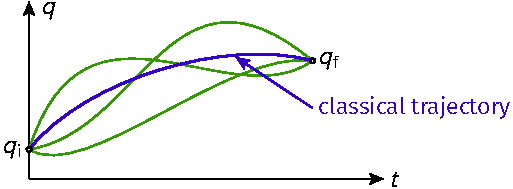
\includegraphics[width=0.6\textwidth]{feynman}
 \end{center}

 \begin{itemize}
  \item All trajectories connecting initial to final point in the given
	time contribute to the propagator.
  \item Almost all of these trajectories are not solutions of the
        corresponding classical equation of motion.
  \item Each trajectory contributes with a phase factor depending on 
	the action associated with the trajectory, cf. double slit.
  \item The nonclassical trajectories can be viewed as contributions
	of quantum fluctuations.
 \end{itemize}
\end{frame}

\begin{frame}[t]{Classical trajectory and\\ quantum fluctuations}
 \vspace{0.4truecm}
 Conventional integral as an analogy:

 \vspace{0.5truecm}
 \begin{columns}
  \begin{column}[b]{0.37\textwidth}
   $S(x)=x^2$
	  
   $x=0$ corresponds to\\[-0.1truecm] classical trajectory

   \vspace{0.8truecm}
   $f(x)=\cos(S(x))$

   \vspace{0.9truecm}
   $I(x)=\int_{-x}^x\text{d}u\cos(S(u))$

   \vspace{0.3truecm}
  \end{column}\hspace{-0.5truecm}%
  \begin{column}[b]{0.6\textwidth}
   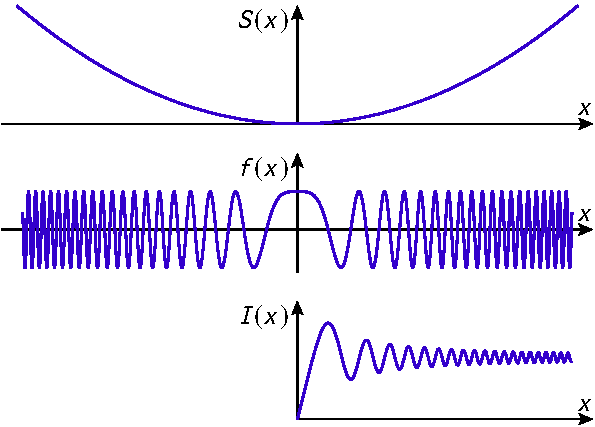
\includegraphics[width=\textwidth]{saddlepoint}
  \end{column}%
 \end{columns}

 The dominant contributions come from stationary points of the action and
 fluctuations around it.
\end{frame}

\section{Particle on a ring}

\begin{frame}[c]{}
 \begin{center}
  \begin{minipage}{0.8\textwidth}
   \tableofcontents[currentsection]
  \end{minipage}
 \end{center}
\end{frame}

\begin{frame}[t]{Standard approach}
 particle of mass $m$ on a ring of radius $R$

 \vspace{0.3truecm}
 Hamiltonian\quad $H = -\dfrac{\hbar^2}{2mR^2}\dfrac{\text{d}^2}{\text{d}\phi^2}$

 \vspace{0.5truecm}
 eigenfunctions with $\psi(0) = \psi(2\pi)$ and $\psi'(0) = \psi'(2\pi)$
 \begin{displaymath}
  \psi_\ell(\phi) = \frac{1}{\sqrt{2\pi}}\text{e}^{\text{i}\ell\phi}\qquad
  \ell = 0, \pm1, \pm2, \ldots
 \end{displaymath}

 eigenenergies
 \begin{displaymath}
  E_\ell = \frac{\hbar^2\ell^2}{2mR^2}
 \end{displaymath}

 propagator
 \begin{displaymath}
  K(\phi_\text{f}, \phi_\text{i}, t) = \frac{1}{2\pi}\sum_{\ell=-\infty}^{+\infty}
	 \exp\left(\text{i}\ell(\phi_\text{f}-\phi_\text{i})
		   -\text{i}\frac{\hbar\ell^2}{2mR^2}t\right)
 \end{displaymath}
\end{frame}

\begin{frame}[t]{More than one way}
 two ways to reach $\phi_\text{f}$:\qquad
	\raisebox{-2truecm}{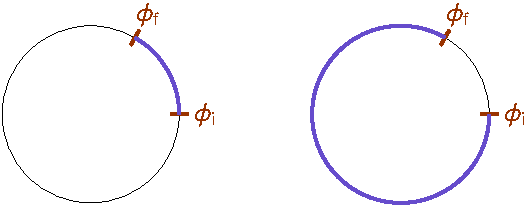
\includegraphics[width=0.6\textwidth]{ring_1}}

 \vspace{0.5truecm}
 \begin{itemize}
  \item the two paths cannot be deformed into each other
 \end{itemize}
 \begin{center}
  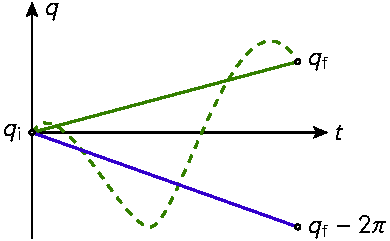
\includegraphics[width=0.53\textwidth]{ring_deform}
 \end{center}
\end{frame}

\begin{frame}[t]{More than one way}
 two ways to reach $\phi_\text{f}$:\qquad
	\raisebox{-2truecm}{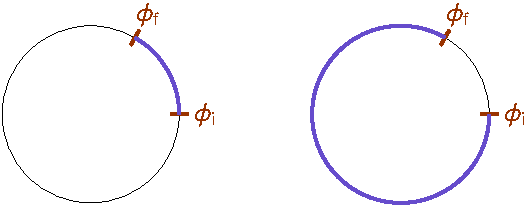
\includegraphics[width=0.6\textwidth]{ring_1}}

 \vspace{0.5truecm}
 \begin{itemize}
  \item the two paths cannot be deformed into each other
  \item two contributions:\\[0.2truecm]
	$R\sqrt{\dfrac{m}{2\pi\text{i}\hbar t}}\exp\left(\dfrac{\text{i}}{\hbar}
		 \dfrac{mR^2}{2}\dfrac{(\phi_\text{f}-\phi_\text{i})^2}{t}\right)$
	\quad and\\[0.2truecm]
	$R\sqrt{\dfrac{m}{2\pi\text{i}\hbar t}}\exp\left(\dfrac{\text{i}}{\hbar}
        \dfrac{mR^2}{2}\dfrac{\big((\phi_\text{f}-2\pi)-\phi_\text{i}\big)^2}{t}\right)$
 \end{itemize}
 \begin{flushright}
  but there is more \ldots
 \end{flushright}
\end{frame}

\begin{frame}[t]{Winding numbers and propagator}
 \begin{center}
  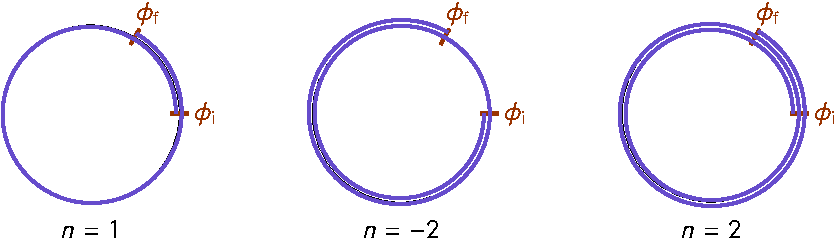
\includegraphics[width=0.8\textwidth]{ring_2}
 \end{center}

 \begin{itemize}
  \item the angles $\phi_\text{f}$ and $\phi_\text{f}+2\pi n$ have
	to be identfied
  \item the propagator is a sum over all topologically distinct contributions
	\begin{displaymath}
	 K(\phi_\text{f}, \phi_\text{i}, t) = R\sqrt{\dfrac{m}{2\pi\text{i}\hbar t}}
         \sum_{n=-\infty}^{+\infty}\exp\left(\dfrac{\text{i}}{\hbar}\dfrac{mR^2}{2}
 	 \dfrac{(\phi_\text{f}-\phi_\text{i}-2\pi n)^2}{t}\right)
	\end{displaymath}
 \end{itemize}
\end{frame}

\begin{frame}[t]{Relating the two representations}
\end{frame}

\section{Particle in a box}

\begin{frame}[c]{}
 \begin{center}
  \begin{minipage}{0.8\textwidth}
   \tableofcontents[currentsection]
  \end{minipage}
 \end{center}
\end{frame}

\begin{frame}[t]{}
\end{frame}

\section{Harmonic oscillator}

\begin{frame}[c]{}
 \begin{center}
  \begin{minipage}{0.8\textwidth}
   \tableofcontents[currentsection]
  \end{minipage}
 \end{center}
\end{frame}

\begin{frame}[t]{}
\end{frame}
\end{document}
